\appendix

\section{Supplementary methods}

\subsection{Data and objective}

\paragraph{Embedding space and data.}
All SONAR models are trained on a fixed cache of $N{=}4{,}000{,}000$
SONAR sentence embeddings ($d{=}1024$, unit-norm) computed from an
interleaved 86-language mC4 sample, with a language label sidecar. The
stream order is deterministic, so raw text is recoverable by row index
(verified against the language sidecar per row). The cloud is unit-normed
but not centred: $\lVert\mathbb{E}[x]\rVert = 0.564$, so it is a
spherical cap and $0.318$ of every squared norm is one shared direction.
It is dense without being isotropic --- effective dimension 108 of 1024
(participation ratio 268 on the whitened eval tail), yet 943 principal
components for 99\% of variance --- and samples average a pairwise cosine
of $0.31$. Sections~\ref{sec:gpt2} and~\ref{sec:seeds} additionally use
GPT-2~\cite{radford2019} layer-8 residual-stream activations ($d{=}768$,
harvested by \texttt{encode\_acts.py}) as a substrate where sparse
dictionary learning is known to work. Section~\ref{sec:gpt2hard} uses a
separate GPT-2 setup from the \texttt{headline} branch --- the residual
stream entering block 8 on FineWeb, unwhitened, scored also by GPT-2 loss
recovered --- whose numbers compare only within that section.

\paragraph{Evaluation.}
All models minimize the whitened MSE of Equation~\ref{eq:mse}. We report
$\fvu$: whitened MSE divided by the whitened variance of a constant
predictor, on the final 32{,}768 cache rows. This tail is excluded from
SAE training and from the training of every straight-through arm.
\emph{Caveat: the softmax Ontologizers (\texttt{resid\_nc} and the
selection sweep) predate the holdout and trained on the full cache
including the tail, so their scores are in-sample; a fresh-encoded
evaluation set is future work.} Where activations are needed, Ontologizer
features are the flattened per-head classification probabilities
$P \in \Delta^{k}{}^{\,l\cdot h}$ at the run's final temperature (feature
$f = (l\cdot h + h_i)k + k_i$; fire threshold $2/k$), and SAE features are
latent activations (fire threshold $0$; runs with softmax heads use the
above-uniform threshold $2/(m/G)$, $G$ heads, matching the entry
convention). Scoring a
softmax run at the default temperature $1.0$ rather than its annealed
$0.03$ puts a healthy checkpoint at $\fvu \approx 0.91$, which is
indistinguishable from a broken one; every number here uses the run's own
temperature.

\subsection{Models and baselines}

\paragraph{Softmax Ontologizers.}
The reference Ontologizer (\texttt{resid\_nc}, step 372{,}600) is the
architecture of Section~\ref{sec:arch}: $l{=}5$ residual layers, $h{=}32$
heads, $k{=}32$ entries per head, bilinear classifiers with residual
normalization and a constant input coordinate, deep supervision, and a
shared linear decoder from an $e{=}2048$ dictionary space; $\approx$23.1M
parameters and $l\cdot h\cdot k = 5{,}120$ dictionary entries. Layers
0--3 trained healthily (prefix $\fvu$ $0.129 \to 0.0051$); layer 4 froze
22/32 heads late in temperature annealing and is mildly harmful
(Section~\ref{sec:lastlayer} explains why). A later \emph{selection sweep}
holds that shape fixed and varies only the \texttt{DictBlock} selection
rule --- \texttt{top1}, \texttt{top2}, \texttt{top4}, \texttt{top8},
\texttt{top16}, \texttt{softmax} --- each with and without the
mean-entropy bonus raised to $s_{\mathrm{KL}_m}{=}3\times10^{-5}$
(\texttt{\_shm}), at 369{,}500 steps.

\paragraph{The straight-through arm.}
\texttt{train\_ste.py} imports \texttt{sonar.py}'s configuration and
overrides only \texttt{select="ste"}: the forward pass selects the argmax
one-hot, and the backward pass uses $\mathrm{softmax}(K/T)$ as its
surrogate. Its shape, calibration and initialization are described with
its results in Section~\ref{sec:ste}.

\paragraph{SAEs.}
SAEs follow Gao et al.~\cite{gao2024}: pre-activation
$\mathrm{relu}((x-b_{dec})W_{enc}+b_{enc})$ with top-$k$ selection,
unit-norm decoder rows, tied initialization, aux-$k$ dead-latent revival,
trained with Adam at $4\times10^{-4}$ for $\sim$144k steps at batch 4096
(converged; convergence is optimizer-step--limited, not epoch-limited, at
this batch size).

\paragraph{The structural-ablation ladder.}
To attribute differences to specific architectural commitments rather than
to whole architectures, we train SAE variants that each add one
Ontologizer-style constraint (all $m{=}5120$, same data and objective):

\begin{center}
\begin{tabular}{@{}llll@{}}
\toprule
rung & run & added structure & analogue \\
\midrule
1  & \texttt{k32} & none (top-$k{=}32$) & baseline \\
2a & \texttt{g160top1} & 160 heads, hard winner per head & heads (hard) \\
2b & \texttt{g160softmax} & 160 heads, softmax per head & heads (soft) \\
3  & \texttt{k32\_p5} & 5 nested prefix losses (matryoshka) & deepsup layers \\
--- & \texttt{k32\_bl} & bilinear encoder, $[x{-}b_{dec};1]$ factors & bilinear classifier \\
\bottomrule
\end{tabular}
\end{center}

Rungs 2a and 2b go far enough that they are no longer SAEs in any
established sense. Per-head competition over a shared decoder is a single
layer of linear classifiers selecting dictionary entries: \texttt{g160top1}
is a one-layer hard-code Ontologizer and \texttt{g160softmax} a one-layer
softmax Ontologizer, each without the bilinear classifier, the residual
stack or the non-negative dictionary. We present them as simplified
Ontologizer variants, not as baselines. \texttt{k32\_bl}'s bilinear encoder
likewise has no standard SAE counterpart, while rung~3 is a Matryoshka-style
SAE.

SAE baselines at width $m{=}11{,}264$ (parameter-matched to the Ontologizer):
\texttt{k32}, \texttt{k160} (coefficient-matched to one deviation per
head), and \texttt{k5120} (coefficient-matched to the full soft code; the
top-$k$ constraint never binds --- measured $L_0 \approx 1520$ --- so it is
effectively a dense ReLU autoencoder). A seed replica \texttt{k32\_s43}
supports stability analysis. The bilinear encoder's latents admit
closed-form ``eigenfeature'' analysis: each latent's symmetric form
$\mathrm{sym}(w_1 w_2^\top)$ is rank~2, with top-$|\lambda|$ eigenvector
$w_1/\|w_1\| \pm w_2/\|w_2\|$ (Pearce et al.~\cite{pearce2025}). Under the
steering frame the simplified variants are the load-bearing comparison:
\texttt{g160softmax} isolates the ``series of softmax classifiers'' idea
from the residual stack, bilinear classifiers and shared dictionary, and
\texttt{g160top1} does the same for hard selection.

\subsection{Evaluation protocols}

Each protocol is a standalone script sharing the eval split and activation
conventions; the root-level ones are unit-tested against planted-structure
synthetic data.

\paragraph{Capacity Pareto (\texttt{pareto.py}).}
Capacity is continuous coefficients transmitted per sample, plus index
bits. Ontologizer code points are \emph{top-$m$ deviation truncations}:
per head, keep the $m$ entries with largest $|p - \mathrm{origin}|$, pin
the rest to the origin distribution, renormalize. The origin is the
corpus-mean classification $\mathbb{E}[p]$ --- measured, not uniform: the
model output is jointly \emph{linear} in the flattened classifications
(zero residual seed, linear decoder), so $\mathrm{decode}(\mathbb{E}[p]) =
\mathbb{E}[Y]$, which decodes to the corpus-mean generic text, while the
uniform code lands off-manifold (cosine $0.067$ to $\mathbb{E}[X]$) ---
despite $\mathrm{KL}_m$ being included in the loss precisely to make the
uniform code the generic one (Section~\ref{sec:labels}). Endpoints:
$m{=}0$ (input-independent origin), $m{=}k$ (exact soft model), and
end-to-end argmax (``hard''). An alternative head-level code mean-ablates
all but the $m$ lowest-entropy heads per layer. SAE points use measured
eval $L_0$. A hard code's index bits are $l\cdot h\log_2 k$; we compare
each against the reverse water-filling bound~\cite{cover2006} on the
whitened eval-tail covariance, the best distortion \emph{any} code of
that rate can reach under a Gaussian model.

\paragraph{Categorical form (\texttt{headstruct.py}).}
An Ontologizer head is exhaustive (always fires) and exclusive (one
winner). We test whether SAE latents form such units: discovery clusters
latents by \emph{paradigmatic} affinity --- similar co-fire profiles with
the rest of the dictionary $\times$ anti-correlation with each other
(PMI${}<1$) --- under a group-size cap, on one half of the rows; scoring
on the held-out half computes per-group exhaustiveness $P(\text{any
fires})$, exclusivity $\mathbb{E}[\#\text{firing} \mid \geq 1]$, and the
CV of summed activation, against size-matched random partitions of the
live-latent pool. Head-like structure requires exhaustiveness \emph{above}
null with exclusivity \emph{below} null; topical co-firing clusters show
the opposite signature. \texttt{--trained-groups} scores a run's own
trained heads instead.

\paragraph{Semantic coherence vs.\ contrast (\texttt{headcoh.py}).}
The complement to categorical form: do a head's entries \emph{mean}
similar things, or do they form a contrast set? Every entry has an exact
decode direction in SONAR output space --- for the Ontologizer, the rows
of the linear map $G$ with $Y = P_{\text{flat}}G$; for SAEs, decoder rows
--- and SONAR space is a semantic sentence space, so within-head direction
similarity is semantic similarity of what entries decode to. Per head we
report mean pairwise cosine and top-singular-value energy fraction,
$z$-scored against size-matched random subsets of the same pool (same
layer for Ontologizer heads); as a metric-hygiene control the same
statistics are recomputed under the training objective's inverse-variance
inner product (\texttt{--metric whitened}). $z \gg 0$ means a head clusters
semantically; $z \ll 0$ means its atoms repel --- the signature of a
\emph{contrastive classifier}, whose entries' atoms are pushed apart. A
second view SONAR-encodes auto-interp description texts and tests pooled
within-head similarity against a label-permutation null.
\texttt{--assignment} scores discovered (post-hoc) groups.

\paragraph{Feature splitting and seed stability (\texttt{splitting.py},
\texttt{partition.py}, \texttt{headcontrib.py}).}
For models $A$ (coarse) and $B$ (fine) on shared rows, each $B$-latent is
classified per $A$-parent by two-way firing containment at threshold
$\tau$: a \emph{child} satisfies $P(A_i \mid B_j) \geq \tau$,
$P(B_j \mid A_i) < \tau$; a \emph{match} satisfies both. Splits
($\geq 2$ children) are scored by union coverage of the parent's firing
set and pairwise child overlap. Decoder geometry adds absorption
candidates (decoder-cosine twins that do not co-fire) and each model's
nearest-neighbour decoder-cosine distribution vs.\ a random baseline. For
two same-architecture runs differing only in seed, the match fractions
are the reproducible-feature fractions. For hard-code Ontologizers,
\texttt{partition.py} matches heads across runs by the NMI of their
partitions (what a head separates), and \texttt{headcontrib.py} by the
cosine of their contributions (what a head writes): each head's decoded
output contribution in the whitened frame, less $\mathrm{decode}(0)$,
centered over rows --- uncentered, the non-negative dictionary's shared
offset reads as agreement. Both use Hungarian matching, a row-shuffled
null, and the same run against an earlier checkpoint as the positive
control. \texttt{headcontrib.py} also splits each head's contribution
size into its layer's input gain and its own decoded atoms, and with a
reference seed pair (a flat arm) compares agreement at matched head size.

\paragraph{Text fidelity (\texttt{textfid.py}).}
The ``loss recovered'' analogue: decode $x$ and $\mathrm{recon}(x)$
through M2M100 (forced \texttt{eng\_Latn}, both rescaled to the reference
SONAR norm, so the metric sees direction error) and report
chrF~\cite{popovic-2015-chrf} and exact-match between the decodes, plus the
decoder's teacher-forced per-token NLL of the \emph{original's} decode
under the original (ceiling), the reconstruction, and the corpus-mean
embedding (floor --- which decodes to the generic text). Under the
steering frame this doubles as the collateral ceiling: a code that cannot
preserve text cannot steer text with low collateral.

\paragraph{Language probing (\texttt{langprobe.py}, \texttt{headlang.py},
\texttt{headscript.py}).}
SAEBench-style $k$-sparse probing with the free 86-language labels: top
latents per language by two-sample $t$-statistic on training rows;
held-out one-vs-rest F1 at $k{=}1$ (single latent, fitted threshold),
$k{=}4,16$ (logistic probes), and a dense probe on the raw embedding as
ceiling. Macro-F1 over languages. \emph{Frame caveat: this measures
whether a factor lives in individual latent magnitudes. A classifier head
carries its factor in its assignment (partition), which single-latent
probes cannot see.} \texttt{headlang.py} is the matching instrument: per
head, the NMI between its partition and the label, null-corrected by a
label shuffle, plus a held-out probe on the best $m$ heads' one-hot
codes against a dense ridge ceiling. NMI here normalizes by the
arithmetic mean of the two entropies, so its attainable maximum is
$2\min(H_h,H_\ell)/(H_h+H_\ell)$ --- $0.875$ for a 5-bit head against the
6.43-bit language label. \texttt{headscript.py} repeats this for script
and scores per-label cells and cross-head conjunctions;
\texttt{headeta.py} measures each partition's $\eta^2$ in embedding
space, corrected by the $(g-1)/(n-1)$ a random $g$-way partition scores.

\paragraph{Shrinkage (\texttt{refit.py}).}
Gao-style refinement: freeze each sample's support, solve the whitened
least-squares coefficients (masked normal equations; silent head slots
forced to zero), and compare $\fvu$. Raw$-$refit is magnitude (shrinkage)
error; refit is selection error. The Ontologizer shares the machinery via
its exact linearity $Y = P_{\text{flat}} G$, with $G$ measured by decoding
one-hot constant codes; its supports are the top-$m$ deviation entries.
Points with support $\geq d$ are excluded (underdetermined). Note the raw
convention: \texttt{refit.py} truncates the soft forward's $P$
(non-adaptive), whereas \texttt{pareto.py} truncates inside the forward,
letting later layers reclassify against the truncated prefix residual.

\paragraph{Steering fidelity in text (\texttt{steerfid.py}).}
Unit-normalized native steering directions --- SAE decoder rows, bilinear
eigenfeatures, or the Ontologizer's \texttt{withArgs} set-intervention
delta --- applied at matched embedding magnitudes. Effect is cycle
consistency: the steered decode is re-encoded through SONAR and the target
feature's activation gain is normalized by its firing-conditioned
quantiles, with the baseline taken from the \emph{cycled} base decode so
both sides share roundtrip degradation. Collateral is $1 - \mathrm{chrF}$
against the base decode. Random unit directions give the control curve,
and \emph{net} effect is feature effect minus that control.

\paragraph{Steering fidelity in embedding space (\texttt{steerembed.py}).}
Drops the text round trip and asks the causal question directly: move
the input along a direction, re-run the model, and record whether the
intended entry is now selected (\emph{realization}) and what fraction of
the \emph{other} heads changed their selection (\emph{collateral}).
Directions: \texttt{decode} (the decode delta of forcing the entry),
\texttt{grad} (the gradient of the target logit), \texttt{margin} (the
gradient of the target's margin over the head's current winner),
\texttt{adjoint} (the bilinear classifier's top eigenvector via
\texttt{BilinearBlock.rev}), and \texttt{random}. 64 entries, 32 held-out
rows each, steered only where the entry was not already selected.

\paragraph{Intervention composition (\texttt{compose.py}).}
Treating heads as candidate causal variables: for pairs of forced
assignments $(l_1,h_1){\to}k_1$, $(l_2,h_2){\to}k_2$ (8 random heads per
layer, one random entry each; all same-layer pairs plus 60 cross-layer
pairs), compare the joint intervention's decode delta $D_{12}$ against
the sum $D_1{+}D_2$ of the single-intervention deltas on 512 held-out
rows: median per-row cosine and relative error
$\|D_{12}-(D_1{+}D_2)\|/\|D_1{+}D_2\|$, raw and whitened. Because the
decode is exactly linear in the flattened classification, final-layer
pairs compose exactly by construction; that stratum doubles as the
measured numerical floor (the $\|R\|{\approx}31 \to \|Y\|{\approx}1$
decoder cancellation amplifies float32 rounding to ${\sim}0.02$ relative
error between differently-compiled variants --- verified exact in
float64). All other non-additivity is downstream reclassification:
later layers re-reading the intervened residual.

\paragraph{Auto-interpretability (\texttt{autointerp.py}).}
Four stages: harvest (top-activating rows, negatives, frequency-stratified
feature selection, parameter-based decode embeddings), texts
(deterministic mC4 stream replay recovers text by row index, verified
against the language sidecar), describe, and score. Description modes:
\texttt{params}, the M2M100 decode of a parameter-derived embedding (for
entries, the $\mathbb{E}[p]$-origin code with one head forced one-hot; for
SAE latents, $b_{dec} + \alpha W_{dec,j}$); \texttt{pdev}, the same decode
with the pure-origin decode subtracted; \texttt{eig}, the bilinear
eigenfeature decode; \texttt{acts}, an LLM summary of top-activating
snippets; and \texttt{cacts}, a \emph{contrastive} summary --- the judge
sees top snippets next to random corpus draws and must name what
distinguishes them, blocking the degenerate corpus-level answer that
plain summaries invite on noisy multilingual web text. Scoring is blinded
detection over held-out positives and negatives, identical for all
modes; per-feature F1, to be read against the always-match null of
$\mathrm{F1} \approx 0.67$ on balanced items. The judge is Haiku
(\texttt{claude-haiku-4-5}) via the Anthropic Messages API, rate-metered,
with bounded reply length; failed judgements are never recorded (an
earlier outage mode scored empty replies as $\mathrm{F1}=0$). Six models:
the Ontologizer, rungs \texttt{k32}/\texttt{k32\_bl}/\texttt{g160top1}/%
\texttt{g160softmax}, and the dense control \texttt{k5120}.

\paragraph{Diagnostic scripts (\texttt{experiments/ste-arm/}).}
The straight-through and geometry results rest on further single-purpose
instruments, described where used: \texttt{inputgeom.py} (geometry of the
vector each classifier sees), \texttt{blendablate.py} (severing the
pairing between a layer's input and the sample's own earlier
reconstruction), \texttt{gainablate.py} (the norm side-channel),
\texttt{dictgeom.py} (row collinearity and effective rank read from the
weights), \texttt{lastlayer.py} (final-layer ablations against the
deep-supervision prefixes), \texttt{decodehead.py} (decoding a head's
atoms as deviations from their mean), \texttt{embedgeom.py} (SONAR
cloud geometry), \texttt{entryshare.py} (how evenly a layer's entries
contribute to the output, and whether usage, gain or atom norm drives the
inequality), and \texttt{bigatoms.py} (how a layer's large atoms are
distributed among its heads, and whether the heads holding them
reproduce).

\section{Supplementary results: the softmax Ontologizer against SAEs}
\label{app:soft}

\subsection{Categorical form}
\label{sec:categorical}

At 1M rows with split-half scoring and 20 size-matched nulls:
\texttt{g160top1}'s trained partition is \emph{perfectly} head-like
(exhaustiveness $1.0000$ vs.\ null $0.64$; exclusivity $1.0000$ vs.\
$1.51$; sum-CV $0.25$ vs.\ $1.03$). Discovery on every unstructured run
(\texttt{m11264\_k32}, \texttt{m5120\_k32}, \texttt{k32\_p5},
\texttt{m11264\_k160}) finds the \emph{opposite} signature ---
exhaustiveness below null ($z$ from $-30$ to $-50$), exclusivity above
($z$ $+13$ to $+31$): spontaneous SAE group structure consists of
co-firing topical clusters, not categorical slots, even when the affinity
explicitly selects for anti-correlated same-context pairs. And
\texttt{g160softmax} never fires distinctly at all: no coefficient ever
exceeds $2/32$ on any test row --- soft per-head codes converge to dense
near-uniform mixtures, exactly as the Ontologizer's soft code does
($\mathbb{E}[p]$ sits $0.06$--$0.16$ bits from uniform in healthy layers;
matching soft reconstruction requires $\sim$16 of 32 deviations per head).
\textbf{Categorical structure exists precisely when trained in as hard
selection, never emerges from softmax competition under a reconstruction
objective, and costs $\sim$60$\times$ in $\fvu$ (0.274 vs.\ 0.0044)
at the SAE's 160 heads.} For steering this means the \emph{soft}
architectures' classifier reading must be cashed out in deviations around
$\mathbb{E}[p]$, not in discrete winners --- or the selection must be
made hard during training, which Section~\ref{sec:ste} does at a far
smaller cost once the head count is raised.

\subsection{Feature reliability}

Seed stability (\texttt{k32} vs.\ \texttt{k32\_s43}; identical
architecture and data, $\fvu$ 0.4994 vs.\ 0.4967): matched-feature
fractions are \textbf{0.31 / 0.24 / 0.15 / 0.03} at
$\tau = 0.3/0.5/0.7/0.9$. Roughly three quarters of individual features
are not reproducible across initializations at moderate containment.
Cross-width splitting (\texttt{k32} $\to$ \texttt{m11264\_k32}): 190 of
5114 live parents split at $\tau{=}0.7$ (median 3 children; union
coverage 0.37; child overlap 0.42), with 441 absorption candidates and a
heavy nearest-neighbour decoder-cosine tail (p50 0.234 vs.\ random
0.119): splitting is real but is not the dominant organization; topical
co-firing is. For a steering generator the unit that must reproduce is
the head's partition rather than the individual feature vector;
Section~\ref{sec:seeds} measures that on the hard-code Ontologizer and
finds it reproduces far \emph{worse} than SAE features do.

\subsection{Text-space fidelity (collateral ceiling)}
\label{sec:textfid}

\begin{table}[h]\centering\small
\begin{tabular}{@{}lrrr@{}}
\toprule
model & chrF & exact & NLL (ceil.\ $\approx$1.56--1.63, floor $\approx$3.8) \\
\midrule
corpus-mean floor & $\approx$0.20 & 0 & 3.60--3.89 \\
k32 tier (incl.\ p5, m11264) & 0.23 & 0.00 & 3.00--3.08 \\
k32\_bl          & 0.21 & 0.00 & 3.19 \\
k160 / g160top1  & 0.28--0.29 & 0.00 & 2.34--2.37 \\
onto soft        & 0.538 & 0.090 & 1.658 (gap 0.026) \\
g160softmax      & 0.592 & 0.119 & 1.563 (gap 0.007) \\
k5120            & 0.856 & 0.592 & 1.587 (gap 0.000) \\
\bottomrule
\end{tabular}
\caption{Downstream text fidelity, 512 tail rows, forced English decodes.}
\end{table}

The FVU--text mapping is sharply nonlinear: $\fvu \approx 0.5$ decodes to
same-topic-different-facts text barely above the generic floor, while the
Ontologizer's soft code and \texttt{g160softmax} are near the likelihood
ceiling --- almost all decodable content survives. Across the eleven
Ontologizer runs with both numbers (the selection sweep and the
straight-through arms; Table~\ref{tab:steerfid}), ``loss recovered'' is a
monotone function of $\fvu$ (rank correlation essentially $-1$), so text
fidelity is a check that the whitened objective transports to text, not
an independent axis --- and it does. This matters doubly under the
steering frame: a steering primitive that routes through a code which
cannot preserve text (the entire $k{\leq}160$ sparse tier) starts from
$\sim$0.75 collateral before any intervention, whereas the dense-mixture
classifier codes start near zero.

\subsection{Concept (language) localization}

\begin{table}[h]\centering\small
\begin{tabular}{@{}lrrrr@{}}
\toprule
model & F1@1 & F1@4 & F1@16 & dense \\
\midrule
k160          & \textbf{0.119} & 0.393 & \textbf{0.473} & 0.676 \\
k32 ($m{=}5120$) & 0.089 & 0.347 & 0.465 & 0.676 \\
m11264\_k32   & 0.078 & 0.364 & 0.471 & 0.676 \\
k32\_bl       & 0.084 & 0.228 & 0.368 & 0.676 \\
g160softmax   & 0.068 & 0.162 & 0.328 & 0.676 \\
g160top1      & 0.066 & 0.200 & 0.302 & 0.676 \\
k32\_p5       & 0.061 & 0.322 & 0.454 & 0.676 \\
k5120         & 0.064 & 0.130 & 0.237 & 0.676 \\
onto (entries) & 0.022 & 0.021 & 0.117 & 0.677 \\
\bottomrule
\end{tabular}
\caption{Macro one-vs-rest F1 over 86 languages, held-out tail.}
\end{table}

Language remains distributed in every model (best single-latent macro-F1
0.119 vs.\ dense ceiling 0.676; script-distinctive languages such as
Chinese reach $\sim$0.98 from one latent, same-script families smear),
and localization \emph{anticorrelates} with reconstruction across the
family. The Ontologizer's entry probabilities are decisively the worst
localizers (F1@1 $=0.022$). Read on SAE terms this is an indictment; read
on classifier terms it is expected: a head encodes a factor in its
\emph{assignment}, not in any single entry's probability, and partition-level
analysis of \texttt{resid\_nc} found layer-1 heads whose partitions carry
script/family mutual information, one of which ((L1,h8,k17)) was causally
verified to force Burmese output. The partition-level instrument
(\texttt{headlang.py}) was later run on a config-matched softmax
reference and on the hard-code arms (Section~\ref{sec:lang}): the softmax
reference's best head reaches a null-corrected NMI of only $0.043$, a
quarter of the hard code's. Language factors are carried by a \emph{few}
heads' partitions, weakly, and most heads classify something else.

\subsection{Shrinkage decomposition}

Top-$k$ SAEs have small magnitude error (share of raw $\fvu$ removed by
support-frozen least squares: 2.2--2.4\% for k32 variants, 8.5\% for
k160, 0.6\% bilinear, 1.9\% p5); \texttt{g160top1} is essentially
perfectly calibrated (0.3\%) --- its reconstruction deficit is pure
selection. The Ontologizer's truncated deviation codes are
magnitude-heavy: 16\% at $m{=}1$, 33\% at $m{=}2$, i.e.\ the
pin-and-renormalize convention mis-scales what it keeps (supports of
$\geq d$ coefficients are excluded as underdetermined). Separately, the
gap between non-adaptive truncation (freeze soft $P$, truncate, decode
linearly) and in-forward truncation (later layers reclassify against the
truncated prefix residual) is large --- $0.268$ vs.\ $0.094$ at $m{=}8$:
downstream layer compensation is worth $\sim$3$\times$ under truncation.
This was the first quantified reconstruction credit for the residual
stack (Section~\ref{sec:depth} measures a larger one), and it is
steering-relevant: the stack actively re-routes around code edits, which
cuts both ways --- robustness to small interventions, and, as
Section~\ref{sec:entangle} shows, widespread collateral.

\subsection{Steering through the text round trip}
\label{sec:steertext}

On the SAE side only a smoke-scale run exists (k32, 3 features):
cycle-consistency effect rises with magnitude (1.2 $\to$ 1.8 over
magnitudes 0.5 $\to$ 1.0 relative to the unit input norm; hit rate 0.67
$\to$ 0.89), while collateral at these magnitudes ($\approx$0.75) is near
the random-direction control. Across the Ontologizer selection sweep and
the straight-through arm, at 64 features per run:

\begin{table}[h]\centering\small
\begin{tabular}{@{}lrrrrrrrr@{}}
\toprule
run & $\fvu$ & chrF & loss rec. & net @0.25 & @0.5 & @1.0 & hit @1.0 & rand.\ hit \\
\midrule
top8          & 0.0370 & --- & 0.940 & 0.131 & 0.303 & \textbf{0.580} & 0.713 & 0.277 \\
top2          & 0.3516 & 0.248 & 0.532 & 0.125 & 0.289 & 0.474 & 0.564 & 0.217 \\
top16         & 0.0052 & --- & --- & 0.065 & 0.119 & 0.243 & 0.313 & 0.139 \\
top8\_shm     & 0.0287 & 0.416 & 0.956 & 0.072 & 0.096 & 0.193 & 0.291 & 0.142 \\
softmax\_shm  & 0.0007 & 0.694 & 0.998 & 0.032 & 0.072 & 0.146 & 0.150 & 0.064 \\
top2\_shm     & 0.1911 & 0.303 & 0.738 & 0.022 & 0.070 & 0.141 & 0.154 & 0.041 \\
top4\_shm     & 0.0761 & 0.360 & 0.897 & --- & --- & --- & --- & --- \\
\texttt{ste\_h76} & 0.2293 & 0.282 & 0.702 & 0.072 & 0.096 & 0.107 & 0.068 & 0.062 \\
top1          & 0.7190 & 0.180 & 0.123 & 0.011 & 0.026 & 0.048 & 0.069 & 0.020 \\
\bottomrule
\end{tabular}
\caption{Text fidelity and text-cycle steering (\texttt{steerfid.py},
\texttt{--n-features 64}) across selection rules. Net effect is feature
effect minus the random-direction control. A further run
(\texttt{topk4\_rev}, $\fvu$ 0.164) reads net 0.520 at 1.0.}
\label{tab:steerfid}
\end{table}

Steerability does not track reconstruction. The best steerer is
\texttt{top8} at $\fvu$ 0.037, the most faithful model
(\texttt{softmax\_shm}) is among the weakest, and every \texttt{\_shm}
variant steers about three times worse than its twin (\texttt{top2} 0.474
vs.\ \texttt{top2\_shm} 0.141; \texttt{top8} 0.580 vs.\ 0.193). The
straight-through arm's effect is positive but nearly flat in magnitude,
and its hit rate (0.068) barely clears its own random control (0.062).
Two cautions on this instrument. Sixteen features is too few to quote: at
16 features the straight-through arm's net effect was negative at every
magnitude and at 64 it is positive throughout. And the hit rate is not
comparable across hard and soft codes: under a hard code an activation
is exactly 0 or 1, so a ``hit'' demands the argmax land exactly on the
target entry, where a soft code need only cross a fractional threshold.

\paragraph{The text cycle is too weak to support conclusions.} Measured on
an \emph{unsteered} round trip (512 held-out rows), the cycled embedding
retains barely more than the shared corpus direction: $\cos(x,
\mathrm{cycle}(x))$ is $0.378$ for \texttt{ste\_h76} and $0.380$ for
softmax, against $0.314$ between random pairs, and a head's argmax
survives the round trip on 12.1\% and 10.5\% of rows against 3.1\%
chance (34.8\% at layer 0, 4.6\% by layer 4 for the hard code). A
perfect intervention could therefore be observed at most $\sim$12\% of
the time --- the same order as the hit rates the instrument reports.
Reconstruction into embedding space is fine; generation is where the
signal goes.

\section{Supplementary results: training, reproducibility and steering of the softmax Ontologizer}
\label{app:softdyn}

These results come from the project proposal's evaluation and concern the
softmax Ontologizer. Two models recur. \texttt{resid\_nc} (372{,}600 steps)
is the reference model behind the softmax tables above.
\texttt{resid\_nc\_hm} is the same configuration plus the batch
mean-entropy bonus $s_{\mathrm{KL}_m}$, trained to 4.38M steps; results
here use its final checkpoint unless stated otherwise.

\subsection{Head freezing and the mean-entropy bonus}
\label{sec:freeze}

A head is counted frozen when its top classification share is at least
$0.95$ and its churn at most $0.02$. In \texttt{resid\_nc} the top layer
(layer 4 of 0--4) begins freezing near step 190k, well after the
temperature anneal, reaches 27 of 32 heads by step 210k and 28 at its
peak, and is still frozen at the last checkpoint
(Figure~\ref{fig:freeze}). Section~\ref{sec:lastlayer} shows the same
layer to be inert once the prefix error is small, which is why the freeze
costs so little reconstruction. In \texttt{resid\_nc\_hm} the late freeze
never occurs. What remains is an early annealing transient --- 22 of 32
heads at layer 1 at step 10k, with 16, 11 and 4 of 32 at layers 2, 3 and 0
--- that recovers completely by step 30k, leaving the final checkpoint
unfrozen everywhere. \textbf{The mean-entropy bonus prevents the late
freeze.}

\begin{figure}[h]\centering
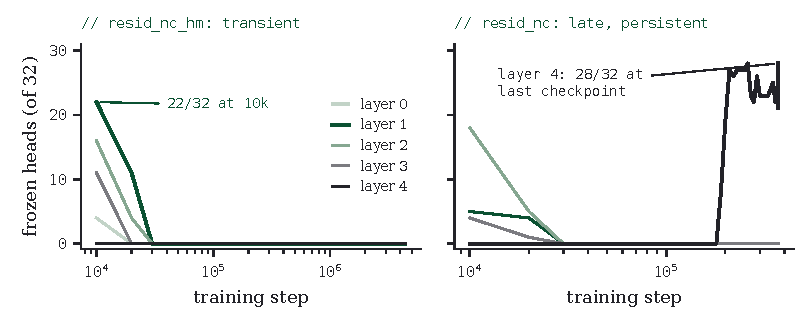
\includegraphics[width=\linewidth]{figures/fig-freeze.pdf}
\caption{Frozen heads per layer over training. Left:
\texttt{resid\_nc\_hm}, with the mean-entropy bonus, has only an early
annealing transient, peaking at 22/32 in layer 1 at step 10k and
recovering to zero everywhere by step 30k. Right: \texttt{resid\_nc}
develops a post-anneal layer-4 freeze from ${\sim}$190k that persists
through its last checkpoint.}
\label{fig:freeze}
\end{figure}

Four retrains of the \texttt{resid\_nc\_hm} configuration (372k steps
each) isolate the transient: a zero-change control and three single-knob
variants. The control reproduces it head for head (22/32 at layer 1 at step
10k, zero everywhere by 30k) and shows no late freeze. Stretching the
temperature anneal from 50k to 150k steps attenuates and spreads it (peak
14/32 at layer 1 at step 30k, clear by 50k). Raising winner dropout from
$0.1$ to $0.25$ tracks the control to within two heads at the peak, and
holding the classification-noise floor at its starting value changes
nothing (Figure~\ref{fig:variants}). The transient belongs to the
temperature schedule alone, and every retrain ends unfrozen.

\begin{figure}[h]\centering
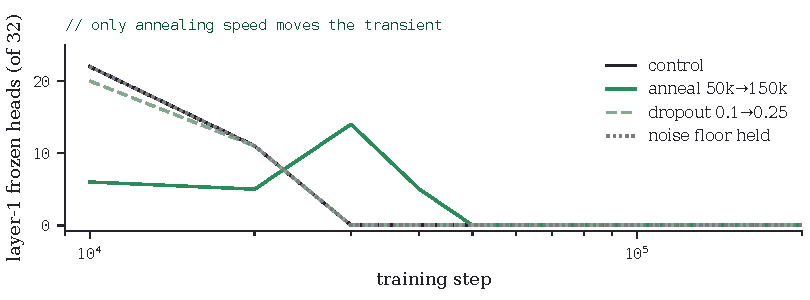
\includegraphics[width=\linewidth]{figures/fig-variants.pdf}
\caption{The early transient under the four retrains, layer-1 frozen
count. The noise-floor variant overlaps the control exactly and the
dropout variant tracks it to within two heads at the peak; only
stretching the temperature anneal moves the curve, trading peak height
for duration.}
\label{fig:variants}
\end{figure}

\paragraph{An HSIC bottleneck in place of the auxiliary losses.} The
candidate objective maximizes dependence with the reconstruction target
while penalizing dependence between heads. It is distinct from the
pairwise head-CKA penalty of Section~\ref{sec:hsic}, which was added to the
straight-through arm's losses rather than replacing them. Both arms were
retrained on the \texttt{resid\_nc\_hm} configuration to 372k steps.
Replacing the four auxiliary terms with the HSIC objective destroys head
health: a late, persistent freeze takes 77 of 160 heads by the final
checkpoint, one layer entirely (layer 3, 32/32 from step 80k), while
reconstruction lands slightly behind the control (tail-mean training MSE
$3.7\times10^{-5}$ against $3.4\times10^{-5}$). Adding HSIC on top of the
auxiliary terms is worse on both counts: MSE $4.4\times10^{-5}$, and 41 of
160 heads still frozen at the end, layer 3 fully frozen by 80k with only
partial thaw (Figure~\ref{fig:hsicbottleneck}). The failure is
\texttt{resid\_nc}'s late freeze rather than the transient, which puts the
bottleneck in direct opposition to the mean-entropy bonus: the bonus
prevents exactly what HSIC induces. As formulated it is neither a
replacement nor an addition.

\begin{figure}[h]\centering
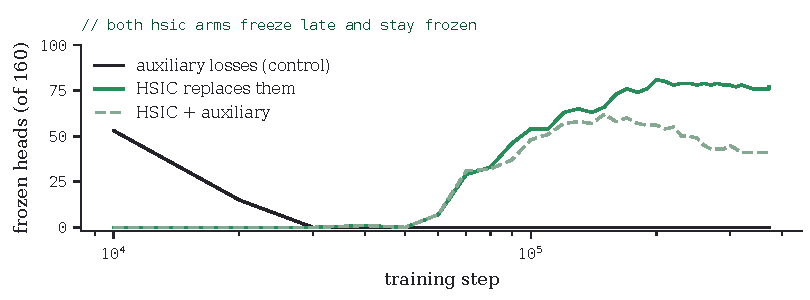
\includegraphics[width=\linewidth]{figures/fig-hsic.pdf}
\caption{Total frozen heads over training for the three loss
configurations, all on the \texttt{resid\_nc\_hm} configuration at 372k
steps. The auxiliary-loss control's freeze is the early transient and
resolves; both HSIC arms develop the late, persistent freeze instead, and
the auxiliary terms only partially thaw it.}
\label{fig:hsicbottleneck}
\end{figure}

\subsection{Development over training}
\label{sec:devinterp}

Tracking \texttt{resid\_nc\_hm}'s full 448-checkpoint history applies the
$z$-score machinery of Section~\ref{sec:prelim-orth} to the refit
end-to-end direction matrix rather than to raw dictionary decode
directions. The two are not directly comparable: raw decode directions on
\texttt{resid\_nc} repel ($z{=}{-}17.6$), while refit directions on
\texttt{resid\_nc\_hm}'s final checkpoint cohere ($z{=}{+}72$); they differ
in both instrument and substrate, and the refit frame folds in the shared
decoder and cross-layer interactions. On that statistic the shape is rise,
peak and partial relaxation (Figure~\ref{fig:devinterp}): mean within-head
$z_{\cos}$ climbs from $1.8$ at step 10k to a peak of $119$ near step 370k
(median $123$, every head above $z{=}2$), then relaxes over the remaining
4M steps to $72$ at the final checkpoint (median $105$, $0.79$ above
$z{=}2$). The code itself moves the other way after the annealing
transient: per-sample entropy returns to $4.5$ of a 5-bit maximum and usage
KL falls toward uniform. Relative to initialization, the consolidation is
in the geometry the classifications write, while the classifications stay
soft.

\begin{figure}[h]\centering
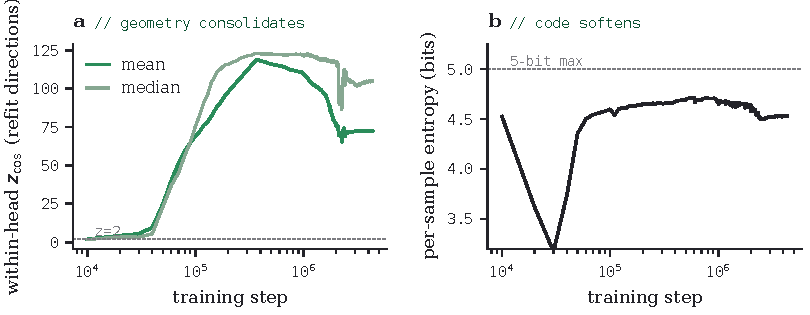
\includegraphics[width=\linewidth]{figures/fig-devinterp.pdf}
\caption{The 448-checkpoint training history of \texttt{resid\_nc\_hm}.
Left: within-head coherence of refit end-to-end directions, $z$-scored
against size-matched nulls; rise, peak near step 370k, partial
relaxation. Right: mean per-sample classification entropy returns toward
the 5-bit maximum after the annealing transient.}
\label{fig:devinterp}
\end{figure}

\subsection{Scaling: a star sweep}
\label{sec:starsweep}

Seven configurations around the shared $h{=}32$, $k{=}32$, $l{=}5$ shape,
varying one axis at a time, each trained 4 epochs (62k steps against the
retrain recipe's 372k), test whether head coherence rises with parameter
count. No measured axis delivers the rise: coherence shows no positive
relation to parameter count (Spearman $+0.14$ for mean $z_{\cos}$, $-0.54$
for the fraction above $z{=}2$), usage imbalance grows with size ($+0.86$),
and the cleanest per-axis trend runs opposite to the prediction, coherence
falling monotonically as entries per head grow ($k{=}16/32/64$: mean
$z_{\cos}$ $20.2/6.3/3.7$). The widest model ($h{=}64$) has not converged at
this budget (tail MSE $20\times$ the others), so its collapse is not
evidence (Figure~\ref{fig:scaling}). Seven points at short training are
weak evidence either way; full-length retrains are the missing control.

\begin{figure}[h]\centering
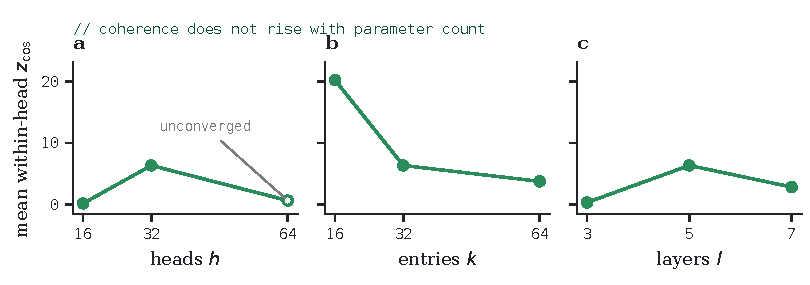
\includegraphics[width=\linewidth]{figures/fig-scaling.pdf}
\caption{Head coherence against each parameter axis of the star sweep,
all runs at 4 epochs (62k steps). No axis delivers the predicted rise;
the entries axis falls monotonically. The open marker is the unconverged
$h{=}64$ run.}
\label{fig:scaling}
\end{figure}

\subsection{Seed stability of soft partitions}
\label{sec:softseed}

A second run of the \texttt{resid\_nc\_hm} configuration from a different
seed, compared at matched training (370k steps on both sides), matches
essentially nothing (Figure~\ref{fig:softseed}): no head pair and at most
$0.3\%$ of atoms clear a $0.3$ cosine threshold on dictionary geometry,
and activation-frame containment over a shared evaluation batch is at most
$0.001$ at any threshold, against $0.31/0.24/0.15/0.03$ for the k32 SAE and
its seed replica across the four thresholds ($0.3$--$0.9$). The metric has
headroom: the same run against itself $2{,}600$ steps apart scores $1.000$
on geometry at every threshold and $0.65$ at the loosest activation
threshold ($0.20$ at the strictest). At matched training the softmax
Ontologizer's partitions are less reproducible across seeds than SAE
latents, the same verdict Section~\ref{sec:seeds} reaches for the
straight-through arm with partition and contribution measures. A replica
carried to the full 4.4M steps is the remaining control.

\begin{figure}[h]\centering
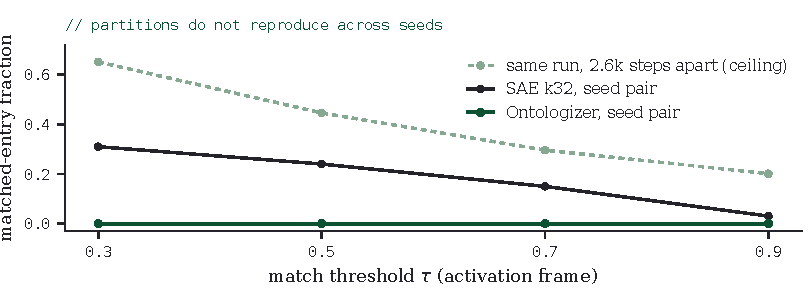
\includegraphics[width=\linewidth]{figures/fig-seed.pdf}
\caption{Cross-seed matched-entry fraction on the activation frame by
threshold. The same-run pair bounds what the metric can detect ($0.65$
at $\tau{=}0.3$); the k32 SAE pair reproduces partially; the softmax
Ontologizer's partitions reproduce not at all.}
\label{fig:softseed}
\end{figure}

\subsection{Steering against supervised baselines}
\label{sec:steeroverlay}

A matched-budget overlay on \texttt{resid\_nc\_hm}'s final checkpoint
compares forced classifications against difference-of-means and
linear-probe directions on language steering, with a random-direction
floor (Table~\ref{tab:steer-overlay}). Each arm wins its own effect frame,
as expected. On the shared difference-of-means frame, forcing a
classification moves decodes along the target direction $0.43\times$ as
far as supervised steering does, and well ahead of probe directions. Every
arm's collateral, supervised steering included, sits at the
random-direction floor ($0.72$--$0.78$), the same floor the text round
trip shows for SAE steering (Section~\ref{sec:steertext}). On naturalness the arms are so far indistinguishable
(Figure~\ref{fig:naturalness}): chrF against unsteered decodes falls from
${\sim}0.35$ at magnitude $0.25$ to ${\sim}0.15$ at $1.0$ for the
difference-of-means and forced-classification arms, with probe and random
decaying in parallel from ${\sim}0.38$ to ${\sim}0.20$. A blinded
human-rating sheet (120 items) is prepared but unscored.

\begin{table}[h]\centering\small
\begin{tabular}{@{}lrrrr@{}}
\toprule
arm & effect (native) & effect (dm frame) & hit rate & collateral \\
\midrule
difference of means    & 0.337 & 0.337 & 0.250 & 0.757 \\
classification forcing & 0.394 & 0.146 & 0.125 & 0.778 \\
linear probe           & 0.293 & 0.028 & 0.000 & 0.720 \\
random direction       & ---   & ---   & ---   & 0.721 \\
\bottomrule
\end{tabular}
\caption{Language steering under matched intervention budgets on
\texttt{resid\_nc\_hm}'s final checkpoint; medians over 24
language--magnitude conditions per arm. Effect is displacement along the arm's
own direction (native) and along the shared difference-of-means direction
(dm frame); hit rate is the fraction of steered decodes reaching the
median projection of genuine target-language rows on the shared frame;
collateral is content change on unrelated dimensions.}
\label{tab:steer-overlay}
\end{table}

\begin{figure}[h]\centering
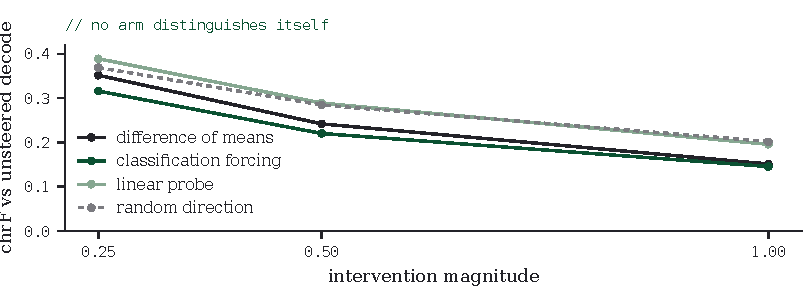
\includegraphics[width=\linewidth]{figures/fig-naturalness.pdf}
\caption{chrF between steered and unsteered decodes by intervention
magnitude. All four arms, the random direction included, damage the
decode at nearly the same rate; no arm buys naturalness at matched
magnitude.}
\label{fig:naturalness}
\end{figure}

\paragraph{A classification as a training objective.} A REINFORCE policy
over steering directions on frozen \texttt{resid\_nc\_hm}, rewarded by one
classification's quantile-normalized score at a matched intervention
budget, converges cleanly in the differentiable in-embedding tier,
saturating within roughly 40 steps at flat collateral
(Figure~\ref{fig:rl}). Neither the decode-cycle tier nor a convergence
race against paired steering has been run.

\begin{figure}[h]\centering
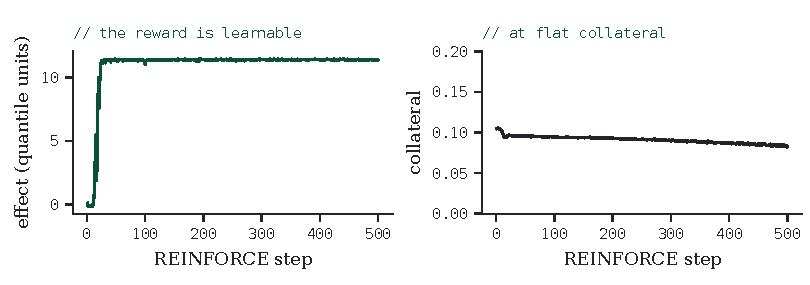
\includegraphics[width=\linewidth]{figures/fig-rl.pdf}
\caption{REINFORCE against a single frozen classification's
quantile-normalized score, in-embedding tier. The policy saturates the
reward within roughly 40 steps while collateral stays at its starting
level.}
\label{fig:rl}
\end{figure}

\subsection{Head-level auto-interpretability}
\label{sec:headautointerp}

The per-latent lenses of the description-specificity results mis-measure
classifier codes, whose content lives in partitions, so a head-level pass
over \texttt{resid\_nc} (step 372{,}600) tests the claim directly; its
frozen top layer (Section~\ref{sec:freeze}) is a caveat for any layer-4
heads in the sample. Descriptions decoded from dictionary parameters fail
at the partition level as they do per latent (median self accuracy
$0.02$). Activation-grounded head descriptions do no better than a null
pairing at this sample size ($n{=}20$ heads per condition, median accuracy
$0.083$ against $0.125$), and a head's detection accuracy is uncorrelated
with the mean describability of its latents (Spearman $+0.07$ over 30
head--lens pairs, 15 heads under each lens; neither per-lens value
distinguishable from zero). The two lenses disagree and neither shows
above-chance head-level signal, so the mis-measurement argument predicts
an advantage this sample does not deliver.

\section{Supplementary results: the straight-through arm}
\label{app:ste}

\subsection{Calibration}
\label{sec:calib}

A naive port (live configuration, \texttt{select="ste"}) trains but the
classifier learns nothing. The root cause is one property: \textbf{the
argmax forward is scale-invariant, so nothing pushes the logits up}; they
sit at their initialization scale (within-head standard deviation
$0.0015$) for the whole run. Three settings follow from it.
\emph{Logit noise must be relative}: $\sigma_K{=}0.02$ is thirteen times
the logit spread, so the argmax is chosen by noise, while $\sigma_K{=}0$
removes the only exploration and the codebook collapses;
\texttt{--noise-k batchnorm} (Equation~\ref{eq:noise_batchnorm}) scales
noise by the logit RMS. \emph{The surrogate temperature must track the
logit scale}: at the live floor $T{=}0.03$, spread$/T$ is 0.05 and the
surrogate is flat, so what improves is the dictionary adapting to a fixed
random partition. \emph{$s_{\mathrm{KL}_m}$ must be rescaled}: $10^{-6}$ is
calibrated against a whitened MSE of $\sim$$3\times10^{-6}$, and a hard
code trains at an MSE orders of magnitude larger, where the term is inert
and heads collapse.

\begin{center}\small
\begin{tabular}{@{}lrrrr@{}}
\toprule
$T$ & spread$/T$ & max $p$ & effective entries/head & raw FVU \\
\midrule
0.01    & 0.15  & 0.043 & 23.4 & 178 \\
0.0015  & 0.78  & 0.135 & 26.4 & 193 \\
0.0005  & 3.38  & 0.681 & 14.0 & 59.2 \\
0.00015 & 16.84 & 0.974 & 3.8  & 7.3 \\
\bottomrule
\end{tabular}
\end{center}

(4000 steps, lr $10^{-5}$, \texttt{--noise-k batchnorm --sd-k 0.3}; one
seed per arm, which ranks configurations but does not predict final
quality.) Sharpening the surrogate is what makes the classifier train at
all and improves reconstruction 25-fold, but it trades directly against
head usage, which $s_{\mathrm{KL}_m}$ exists to hold. At \texttt{sonar.py}'s
learning rate $5\times10^{-5}$ every sharp-surrogate arm collapsed
abruptly after $\sim$1700 steps; $10^{-5}$ is stable. The shipped arm is
$T{=}1.5\times10^{-4}$, lr $10^{-5}$, \texttt{--noise-k batchnorm
--sd-k 0.3}, $s_{\mathrm{KL}_m}{=}10^{-4}$, trained 24 epochs
(369{,}500 steps). The temperature is hand-matched to a logit scale
measured once; the principled version normalizes logits per head or
controls $T$ against a spread$/T$ setpoint.

\subsection{Capacity beyond bits, and training dynamics}

\paragraph{Bits are not the whole capacity.} At identical bits, 380
binary heads reach $0.1844$ against 76 thirty-two-way heads at $0.1535$:
bits go as $h\log_2 k$ but the codebook goes as $h\cdot k$ (3800 atoms
against 12{,}160). The binary arm gets within 17\% on $2.9\times$ fewer
parameters, with features that are one bit each --- the form that is
actually nameable.

\paragraph{Training dynamics.} On the shipped arm, reconstruction
converges early (MSE flat from step 237k) while within-head row
collinearity keeps falling ($0.812 \to 0.686$, against $\sim$0.64 for
random non-negative rows) and head-usage imbalance $\mathrm{KL}_m$ falls
from a 14.8-bit peak near step 5k to 2.71. The $s_{\mathrm{KL}_m}$
rescale is what turns the usage peak around.

\subsection{Depth: eliminations and mechanism}
\label{sec:depthdetail}

The comparison went through two wrong versions first, and the
eliminations are informative. On the shipped initialization the flat arm
read $0.5822$ at 484 realized bits (25.5\%), a $2.5\times$ gap. Correcting
the per-head entropy pressure --- $\mathrm{KL}_m$ averages over a layer's
heads and the loss sums over layers, so per-head pressure scales as
$s_{\mathrm{KL}_m}/h$ per layer and the flat arm had trained at a fifth of
the stack's --- took it to 1199 bits and $0.4307$. A frozen ZCA whitener
(\texttt{make\_zca.py}) took the classifier's input from effective
dimension 107 to 901 and the code to 1900 of 1900 bits, every head at
4.999 of 5 bits, more than the stack itself realized --- and still
reconstructed $1.7\times$ worse ($0.3842$). Two survivors from that line:
\textbf{usage is not what depth buys} (bits are not the objective either:
dropping $s_{\mathrm{KL}_m}$ 100$\times$ costs the stack 176 bits and
\emph{improves} its error to $0.2095$), and \textbf{a learned input
transform collapses where a supplied one does not} --- a jointly trained
\texttt{Linear} encoder ends with every head on exactly two entries at
$\fvu$ $0.6853$, worse than no encoder.

\paragraph{The input each classifier sees.} \texttt{inputgeom.py}, on the
exact vector handed to each classifier (shipped arm):

\begin{center}\small
\begin{tabular}{@{}lrrr@{}}
\toprule
layer & mean direction & mean pairwise cos & effective dim / 1024 \\
\midrule
0 & 0.5638 & 0.3146 & 107.5 \\
1 & 0.0932 & 0.0087 & 611.3 \\
2 & 0.1522 & 0.0233 & 596.3 \\
3 & 0.1983 & 0.0396 & 548.8 \\
4 & 0.2348 & 0.0553 & 507.1 \\
\bottomrule
\end{tabular}
\end{center}

Layer 0 (and every flat arm) classifies the raw cap; layers 1--4 classify
residuals that span over half the space. On the shipped arm, layer 0 was
the only layer that did not fill its code (10.6 live entries, 216 bits,
against $\sim$375 for each later layer) --- a within-model control on
everything except the input.

\paragraph{What the cascade contributes: pairing.}
\texttt{blendablate.py} blends the subtracted term
$\mathrm{decode}(R_i)$ in layer $i{+}1$'s input toward a reference with
the same marginals and none of the pairing --- another row's
reconstruction (shuffle), the mean, or Gaussian noise rescaled to the
shuffle's per-sample magnitude --- without retraining:

\begin{center}\small
\begin{tabular}{@{}lrrrrr@{}}
\toprule
blend & shuffle & mean & noise & eff.\ dim L1 (shuffle) & (noise) \\
\midrule
0.000 & 0.2292 & 0.2292 & 0.2292 & 499.1 & 499.1 \\
0.125 & 0.2460 & 0.2374 & 0.2426 & 476.0 & 504.7 \\
0.250 & 0.3084 & 0.2652 & 0.2838 & 394.2 & 518.3 \\
0.500 & 0.6910 & 0.4100 & 0.4665 & 193.4 & 539.6 \\
0.750 & 1.8154 & 0.7497 & 0.8502 & 103.0 & 527.6 \\
1.000 & 4.6613 & 1.4302 & 1.5992 & 68.5 & 496.2 \\
\bottomrule
\end{tabular}
\end{center}

The pairing is load-bearing well below full severance --- a quarter blend
costs 35\% of $\fvu$ --- and another row's reconstruction does more damage
than matched-magnitude noise at every level, so the damage is specific
rather than generic perturbation sensitivity. The sweep cannot separate
pairing from conditioning: effective dimension falls in lockstep with the
error, because a residual is small and nearly isotropic \emph{because} it
is this sample's own error. That resolves the whitened arm rather than
conflicting with it: whitening is conditioning without pairing, and it
bought full utilization and $\sim$7\% of $\fvu$. (\texttt{forward="labels"},
which would test this by removing the residual entirely, has not been run
at the fixed initialization. Forwarding the code \emph{alongside} the
residual, \texttt{forward="resid\_labels"}, was a clear negative in a
three-epoch pilot: held-out $\fvu$ $0.826$ against $0.249$, after leading
early by $50\times$ --- the signature of a parameter advantage without an
information advantage, since the residual is by construction what the
code failed to explain.)

\paragraph{The code is not the whole channel.} Each layer splits its input
into a unit direction (all the classifier sees) and a norm that multiplies
the layer's output, so one real number per layer per sample reaches the
decoder outside the bottleneck. Pinning each gain to its held-out mean
(\texttt{gainablate.py}) costs the stack $+2.1\%$ in total (layer 0's
gain is identically 1, since SONAR is unit-norm), against a 68\% gap: the
channel is real and is not the explanation. It does matter as a confound
for the whitened flat arm, whose whitener creates a varying layer-0 gain
worth $+4.5\%$ --- about 40\% of whitening's apparent benefit.

\paragraph{The decoder is dense, and not because of the offset.}
Magnitude-pruning the trained decoder's smallest half takes $\fvu$ into
the thousands, and its weight distribution looks like a Gaussian
matrix's. The non-negative dictionary makes $R$'s constant part dwarf its
varying one ($\lVert\mathbb{E}R\rVert / \mathbb{E}\lVert R-\mathbb{E}R
\rVert = 11.6$), and the bias-free decoder does attenuate that constant
to the embedding mean (norm 0.581 against 0.564). But a decoder bias
(\texttt{--biased-dec}) is worth only $-0.62\%$ of training MSE at matched
step (the run died at 23\% of its schedule, so its held-out $0.2464$ is
not comparable to the converged arm's): pinning
$W\,\mathbb{E}R$ is 1024 linear constraints on a $1024\times2048$ matrix,
0.05\% of its freedom. The decoder is dense because a full-rank map
carrying a $\sim$900-dimensional signal is dense.

\subsection{Steering by target layer, and head-health levers}
\label{sec:steerlayer}

Splitting the stack's steering by target layer (strength 1.0, 12 entries
per layer) reverses the aggregate ranking of directions:

\begin{center}\small
\begin{tabular}{@{}lrrrrr@{}}
\toprule
layer & decode & grad & margin & adjoint & random \\
\midrule
0 & 0.216 & \textbf{0.583} & 0.547 & 0.237 & 0.034 \\
1 & 0.464 & 0.089 & 0.367 & 0.000 & 0.023 \\
2 & 0.742 & 0.130 & 0.216 & 0.000 & 0.055 \\
3 & \textbf{0.966} & 0.130 & 0.091 & 0.000 & 0.034 \\
4 & 0.362 & 0.047 & 0.036 & 0.005 & 0.047 \\
\bottomrule
\end{tabular}
\end{center}

Where the input reaches the classifier directly (layer 0), the
classifier's own geometry (\texttt{grad}, \texttt{margin}) beats
\texttt{decode} three- to tenfold. With depth it fails: a direction
computed against layer $i$'s classifier input is only valid there, and
the perturbation arrives after earlier layers have re-encoded it. The
\texttt{decode} direction moves the input toward what the model itself
emits with the entry active, which is self-consistent down the stack. Layer
4 is hard for everything: its residual is nearly exhausted. The practical
reading is to steer layer 0 by gradient and the middle layers by decode.

\paragraph{Head-health levers and steering.} Three levers were tried on
the shipped stack. \emph{Mean-entropy pressure is not what costs
steerability}: a twin trained at $s_{\mathrm{KL}_m}{=}10^{-6}$ has raw
text-cycle effect $0.039$ against $0.029$, both an order of magnitude
below \texttt{top2}/\texttt{top8} at the same weight, so hard selection,
not the bonus, is the cost (removing the bonus does cost head usage:
imbalance 5.00 bits against 2.71). \emph{Head-independence pressure
(HSIC/CKA) was chasing estimator bias} (Section~\ref{sec:hsic}).
\emph{A row-collinearity setpoint is the one lever that bought
steerability}: holding within-head row cosine at 0.5 (against an
uncontrolled 0.774) improves embedding-space realization in every
direction at lower collateral --- \texttt{decode} $+15\%$,
\texttt{grad} $+17\%$, \texttt{margin} $+52\%$, oriented
\texttt{adjoint} $+122\%$, collateral 0.591 $\to$ 0.552 --- with held-out
$\fvu$ slightly better ($0.2157$ vs.\ $0.2293$). The controller holds its
setpoint as a thermostat: the dual multiplier is projected to zero while
the constraint is satisfied. Its mechanism is unexplained: the
statistic is computed in the $e$-dimensional dictionary space, where
74--78\% of each atom's energy is in the decoder's null space
(Section~\ref{sec:rowcos}), and decoded the atoms were already
orthogonal. That the classifier-geometry directions gain most suggests
an effect on the classifier rather than the dictionary, but nothing
establishes it. The setpoint does not transport to the flat arm, whose
steering is already saturated (0.992 vs.\ 0.966).

\subsection{Head independence: a measurement artifact}
\label{sec:hsic}

A head-independence penalty (\texttt{--s-hsic-heads}, pairwise head
CKA~\cite{kornblith2019}) appeared to find substantial dependence. It was
measuring bias:

\begin{center}\small
\begin{tabular}{@{}lrrrrrr@{}}
\toprule
layer & 0 & 1 & 2 & 3 & 4 & mean \\
\midrule
unbiased & 0.0041 & 0.0005 & 0.0005 & 0.0004 & 0.0002 & \textbf{0.0011} \\
biased   & 0.0315 & 0.1062 & 0.1018 & 0.0963 & 0.0976 & 0.0867 \\
\bottomrule
\end{tabular}
\end{center}

The biased estimator reads chance co-occurrence between independent
categorical heads as dependence, with a floor that grows as the batch
shrinks (0.109 at $b{=}256$, 0.029 at 1024, against an unbiased 0.0001 at
every size). At the training batch the floor exceeded any real
dependence, so the penalty had nothing to descend but the bias.
\texttt{hsic.pairwise\_head\_cka} now defaults to the unbiased
estimator~\cite{song2012}, which reads 0.06 at 0.5 planted factor
correlation and 0.41 at 0.8. Conditioning on language or script explains
none of the residue. \textbf{This architecture produces near-independent
heads with no pressure to do so}; trained out under the corrected
estimator the penalty changes nothing and costs localization
(best-head language NMI 0.199 against 0.269). Two lessons generalize:
before trusting a statistic as a training signal, measure it on a null
it should score zero on; and loss-value share is not gradient share ---
at $s{=}10^{-4}$ the penalty was 12\% of the loss value, while the
measured MSE-to-CKA gradient ratio (1250 at the classifier, 221 at the
dictionary) put equal pull at $8\times10^{-4}$.

\subsection{Seed reproducibility, measure by measure}
\label{sec:seedsdetail}

\emph{Partitions.} The best-matched pair of heads reaches NMI 0.42, but
the mean is 0.012 against a 0.005 null, and \texttt{splitting.py}'s entry
containment reads 0.000. Neither is a metric artifact: comparing one run
against its own checkpoint 19{,}500 steps earlier, the same partition
measure scores 0.38 overall and 0.87 on layer 0. \emph{Contributions.}
Two heads could carve differently and add the same thing; they do not
(centered cosine 0.0074 vs.\ 0.0015 null; uncentered it reads 0.205, which
is the non-negative dictionary's shared offset). \texttt{headcontrib.py},
which fixes the measurement (decoded, whitened, centered contributions,
Hungarian-matched), reads $0.019$ against a $0.0017$ null on the same
pair at 4{,}096 rows; the earlier one-off figure's exact method was not
recorded, and the conclusion is unchanged under either. \emph{Subspaces.}
Top-8 eigenspaces of per-layer contributions agree 25--33$\times$ above
chance --- but each model agrees with the \emph{cache's own} principal
directions by the same amount (e.g.\ layer 1: 123.7$\times$ between
seeds, 101.3$\times$ and 101.2$\times$ to the data), so the agreement is
the data's and nothing is left for the architecture. At layer 4 each
seed tracks the data $\sim$23$\times$ above chance while agreeing with the
other only 9$\times$: they pick \emph{different} data-aligned directions.
\emph{Grams.} Per-layer row collinearity agrees to four digits (0.2880 /
0.2891 at layer 0), but the Gram spectrum is nearly one-parameter --- the
top eigenvalue is exactly $1+(k-1)\,\mathrm{rowcos}$, carries 82\% of the
spectrum's norm, and is forced by non-negativity. Compared entrywise in
canonical order, Grams agree at chance across seeds (1.05--1.11$\times$)
and \emph{equally} at chance against the same run 19{,}500 steps earlier
(1.07--1.15$\times$): a head's Gram is close to a fixed property of the
configuration rather than something learned. Decoding atoms to output
space first changes nothing (1.18$\times$ at layer 0 to 1.03$\times$ at
layer 4).

\subsection{What makes layer 0 reproduce: gain, atoms, and depth}
\label{sec:l0size}

Layer-0 heads are the largest and the most reproducible, so ``layer 0
reproduces'' might be ``large heads reproduce''. \texttt{headcontrib.py}
measures a head's size as its centered contribution energy over the
whitened target variance, and splits it exactly: a head's contribution on
a row is its layer's input gain times the decoded atom it selected, so
its size is gain$^2$ times atom spread$^2$ (the usage-weighted RMS
distance of its decoded atoms from their mean); on both stacks the
product reproduces the measured size to a log correlation of 1.000.

\begin{table}[h]\centering\small
\begin{tabular}{@{}lrrrrrr@{}}
\toprule
& \multicolumn{3}{c}{GPT-2 concat} & \multicolumn{3}{c}{SONAR stack} \\
layer & agreement & gain & atom norm ($10^{-4}$) & agreement & gain & atom norm \\
\midrule
0 & 0.171 & 122.2 & 4.6 & 0.080 & 1.000 & 0.043 \\
1 & 0.017 & 67.9 & 5.3 & 0.005 & 0.588 & 0.054 \\
2 & 0.007 & 62.3 & 4.4 & 0.004 & 0.490 & 0.052 \\
3 & 0.005 & 59.2 & 3.7 & 0.003 & 0.417 & 0.051 \\
4 & 0.004 & 57.2 & 3.2 & 0.003 & 0.359 & 0.043 \\
\bottomrule
\end{tabular}
\caption{Head agreement (matched centered contribution cosine) and the
two factors of head size, medians over each layer's heads; atoms decoded
and whitened. SONAR: \texttt{ste\_h76\_init01} against
\texttt{ste\_h76\_i01\_s43}, 4{,}096 rows.}
\label{tab:gainatoms}
\end{table}

\textbf{Layer 0's larger contributions are all gain.} It receives the raw
input --- GPT-2 activations of norm $\sim$122 against residuals of
$\sim$60; unit SONAR embeddings against residuals of 0.36--0.59 --- while
its atoms are no larger than layer 1's on either dataset, and on SONAR
smaller than those of layers 1--3 and equal to layer 4's. Gain is one
number per layer per row, shared by all of a layer's heads, so across
layers ``size'' is the layer itself under another name. At equal atom
spread, layer 0 still reproduces $14\times$ better on GPT-2 and $23\times$
better on SONAR (log agreement on log spread and a layer-0 indicator,
$R^2$ 0.979 and 0.941).

\paragraph{Against the flat arm at matched size.} Within a stack, head
size and layer do not overlap, so their effects cannot be separated
there. The flat arm breaks the confound: all its heads see the raw input,
with gain 1 and nothing downstream. On SONAR its own agreement tracks
log head size at $r = 0.876$ --- from $0.008$ for its smallest heads
(0.057--0.060\% of target variance) to $0.150$ above 0.071\%, and $0.78$
and $0.56$ for its two largest --- so size matters a great deal on its
own, and since its gain is constant it is an atom-magnitude curve. But
the stack's heads fall far below that curve at every depth, layer 0
included:

\begin{center}\small
\begin{tabular}{@{}lrrrr@{}}
\toprule
stack layer & size, median & stack agreement & flat heads at that size ($\pm$10\%) & gap \\
\midrule
0 & 0.31\% & 0.080 & 0.67 ($n{=}2$) & $\sim$8$\times$ \\
1 & 0.16\% & 0.005 & 0.12 ($n{=}1$) & $\sim$23$\times$ \\
2 & 0.11\% & 0.004 & 0.19 ($n{=}3$) & $\sim$49$\times$ \\
3 & 0.073\% & 0.003 & \textbf{0.059} ($n{=}115$) & $\sim$\textbf{19}$\times$ \\
4 & 0.039\% & 0.003 & below the flat range & --- \\
\bottomrule
\end{tabular}
\end{center}

\textbf{The stack costs reproducibility at matched size, at every
layer.} Layer 0 sees exactly the flat arm's input and still reproduces
several times worse than an equal-size flat head: in the stack, what a
layer-0 head should carve depends on what the layers after it do with
its error, so the input alone no longer pins it. Deeper layers lose
more. This is the reproducibility face of the entanglement result
(Section~\ref{sec:entangle}): the cascade that doubles a single-head
intervention's collateral, to 66\% of the other heads, also leaves each
head underdetermined by the data. Read against the flat curve, the gain
difference between layers 0 and 3 accounts for roughly a third of layer
0's lead in log terms; only layer 3's size match is solid --- flat heads
are almost all small, so layers 0--2 rest on one to three heads each ---
so the fraction is rough and the direction firm. The matched-size
comparison is SONAR-only; GPT-2 has no flat arm.

\paragraph{Within layer 0 the atoms decide.} SONAR's layer-0 gain is
identically 1, so its within-layer size variation is pure atom
magnitude, and there log agreement tracks atom norm at $r = 0.62$ and
spread at $0.64$ (cosine against log size, $0.91$); GPT-2's layer 0 shows
$0.17$ and $0.42$. Past layer 1 the atoms predict nothing on either
dataset. Spread and norm are one quantity here --- their ratio is
0.99--1.08 in every layer, so a head's usage-weighted mean decoded atom
is near zero: the non-negative dictionary's offset is cancelled by the
decoder before it reaches the output.

\subsection{How entries share a layer}
\label{sec:entries}

An entry writes only where it wins its head, and then writes its layer's
gain times its decoded atom, so its energy over the data is
$\mathbb{E}[\mathbf{1}\{\text{selected}\}\,\mathrm{gain}^2]\,
\lVert\text{atom}\rVert^2$. Per layer, over 32{,}768 held-out rows
(\texttt{entryshare.py}):

\begin{table}[h]\centering\small
\begin{tabular}{@{}llrrrrr@{}}
\toprule
run & layer & Gini & top 10\% carry & max/median & from atom norm & within heads \\
\midrule
GPT-2 concat, $k{=}256$ & 0 & \textbf{0.587} & 42\% & 38.7 & 76\% & 60\% \\
& 1 & 0.155 & 16\% & 30.3 & 44\% & 100\% \\
& 2--4 & 0.11--0.12 & 14\% & $\sim$2 & $\sim$40\% & 100\% \\
SONAR stack, $k{=}32$ & 0 & \textbf{0.326} & 32\% & 46.3 & 92\% & 83\% \\
& 1--3 & 0.06--0.10 & 12--14\% & 1.5--1.9 & 16--24\% & $\sim$100\% \\
& 4 & 0.195 & 18\% & 3.2 & 77\% & 87\% \\
SONAR flat, $1\times380$ & --- & 0.190 & 23\% & 64.1 & 90\% & 76\% \\
\bottomrule
\end{tabular}
\caption{Inequality of entry energy within a layer. ``From atom norm'' is
the covariance share of the variance of log entry energy (the remainder
is usage; gain conditional on selection contributes $\sim$0). ``Within
heads'' is the share of that variance not explained by which head an
entry is in. No entry is dead in any layer.}
\label{tab:entries}
\end{table}

\textbf{Layers 1--3 are near-equal; layer 0 is not, and its atoms are
why.} Deep entries have an effective number of 95--99.5\% of the total
and the largest is about twice the median; what inequality they have is
mostly usage, itself mild (CV 0.14--0.18). Layer 0's usage is just as
even --- on SONAR every entry fires 2.1--4.5\% of the time against $1/k =
3.1\%$ --- but its atom norms vary five to ten times more (CV 0.34--0.52
against 0.02--0.10), mostly inside heads. The flat arm shows the same
pattern more mildly, so it belongs to classifying the raw input. SONAR's
last layer is unequal for the other reason: some atoms have shrunk almost
to nothing (smallest/median 0.017), the inert final layer of
Section~\ref{sec:lastlayer}. Whole layers are unequal by gain: layer 0
holds 67\% of entry energy on GPT-2 and 49\% on SONAR, layer 4 4--5\%.

\paragraph{Where the large atoms sit} differs completely between the
models (\texttt{bigatoms.py}):

\begin{center}\small
\begin{tabular}{@{}lll@{}}
\toprule
& GPT-2 concat, 20 heads & SONAR stack, 76 heads \\
\midrule
\multicolumn{3}{@{}l}{\emph{within a head} (atom norm $/$ the head's own median, mean over heads)} \\
\quad largest & 3.7 (1.4--5.1 across heads) & 2.0 (1.5--4.3 across heads) \\
\quad 2nd / 8th / 16th largest & 3.2 / 2.0 / 1.7 & 1.7 / 1.2 / 1.0 \\
\quad largest entry's share of head energy & 6.1\% (uniform 0.4\%) & 9.9\% (uniform 3.1\%) \\
\multicolumn{3}{@{}l}{\emph{across the layer} (atom norm $/$ the layer median)} \\
\quad atoms $>2\times$ & 1030 (20\%), in all 20 heads & 63 (2.6\%), in 28 heads \\
\quad atoms $>3\times$ & 58, in \textbf{all 20} heads (at most 15 each) & 11, in \textbf{4} heads \\
\quad atoms $>5\times$ & 1 & 5, \textbf{all in head 54} \\
\quad largest head's energy share & 15.5\% (3$\times$ uniform) & 9.2\% (7$\times$ uniform) \\
\multicolumn{3}{@{}l}{\emph{usage}} \\
\quad Spearman(atom norm, usage) in heads & $+0.81$ & $+0.27$ ($-0.04$ to $+0.58$) \\
\quad usage of atoms $>3\times$ / of the rest & 0.0062 / 0.0037 ($1/k$ 0.0039) & 0.033 / 0.031 ($1/k$ 0.031) \\
\multicolumn{3}{@{}l}{\emph{direction}} \\
\quad $|\cos|$ between heads' largest atoms & 0.022 (random pairs 0.048) & 0.023 (random pairs 0.028) \\
\quad energy in the data's top 10 PCs & 4\% (all atoms 13\%) & 9\% (all atoms 3\%) \\
\bottomrule
\end{tabular}
\end{center}

On GPT-2 every head has a graded tail --- its eighth-largest atom is
still twice its median --- and the large atoms are its frequent outcomes
(1.6$\times$ uniform usage). Agreement is fairly even across heads
(0.135--0.235) and only loosely tied to atoms (Spearman 0.49 with energy
share, 0.34 with the largest atom). On SONAR the large atoms are a few
heads' property, and fire at the uniform rate: large, not frequent. Head
54 holds 8 of the 11 atoms above $3\times$ and all 5 above $5\times$,
carries 9\% of the layer, and reproduces at \textbf{0.844} against 0.249
for the next head; across heads, agreement tracks the largest atom
(Spearman 0.62) and how peaked the head's profile is (0.62), not its
typical atom ($-0.14$). That resolves the within-layer-0 atom effect into
a few heads with outsized atoms --- but not the layer-0 lift: without head
54 the layer-0 mean falls only from 0.080 to 0.070, still twenty times
the deep layers. Head 54 is the topic/genre head of
Section~\ref{sec:lang}, which recurs across seeds.

\begin{table}[h]\centering\small
\begin{tabular}{@{}lrrrrr@{}}
\toprule
head & agreement & energy share & largest $/$ layer median & atoms $>3\times$ & largest $/$ head median \\
\midrule
\multicolumn{6}{@{}l}{\emph{SONAR stack, layer 0} (uniform share 1.3\%)} \\
54 & \textbf{0.844} & 9.2\% & 6.81 & 8 & 3.41 \\
46 & 0.249 & 2.5\% & 3.21 & 1 & 2.24 \\
6  & 0.181 & 1.5\% & 2.76 & 0 & 2.83 \\
18 & 0.150 & 1.9\% & 4.50 & 1 & 4.34 \\
\quad lowest four & 0.008--0.021 & 1.0--1.1\% & 1.51--1.84 & 0 & 1.48--1.84 \\
\midrule
\multicolumn{6}{@{}l}{\emph{GPT-2 concat, layer 0} (uniform share 5\%)} \\
6  & 0.235 & 3.1\% & 4.31 & 2 & 4.77 \\
17 & 0.220 & 15.5\% & 4.99 & 5 & 1.90 \\
19 & 0.215 & 3.4\% & 3.82 & 3 & 4.16 \\
0  & 0.202 & 3.1\% & 3.95 & 1 & 4.19 \\
\quad lowest four & 0.135--0.141 & 2.6--3.0\% & 3.13--4.17 & 1--2 & 3.45--4.56 \\
\bottomrule
\end{tabular}
\caption{Layer-0 heads by seed agreement (\texttt{bigatoms.py}; matched
centered contribution cosine against the seed-43 twin). Spearman of
agreement across heads, SONAR / GPT-2: with energy share $+0.53$ /
$+0.49$; with the largest atom $+0.62$ / $+0.34$; with the head's peakedness
(largest $/$ head median) $+0.62$ / $+0.09$; with its median atom $-0.14$ /
$+0.16$.}
\label{tab:bigatoms}
\end{table}

The two models differ in kind here. On SONAR one head stands out on every
atom measure and alone reproduces strongly; the rest of layer 0 is a
long, nearly flat tail, and agreement follows how peaked a head's atoms
are. On GPT-2 no head stands out: every head has several large atoms, the
spread of agreement is narrow, and the head with the largest share of the
layer's energy (17) has a flat profile --- uniformly large atoms rather
than a few outsized ones --- yet reproduces no better than its
neighbours. Peakedness predicts nothing there ($+0.09$).

The large atoms are distinct directions: different heads' largest atoms
are near orthogonal (median $|\cos|$ 0.022--0.023, below random atom
pairs). On SONAR they lean into the data's top ten principal directions
(9\% of their energy against 3\% for a typical atom), consistent with
cross-seed agreement being the data's dominant directions; on GPT-2 they
lean the other way (4\% against 13\%). One seed pair per dataset
throughout.

\subsection{Language: the probe in detail}
\label{sec:langdetail}

Held-out language identity over 86 languages (dense ridge ceiling 0.721,
chance 0.012):

\begin{table}[h]\centering\small
\begin{tabular}{@{}llrrrr@{}}
\toprule
arm & shape & best-head NMI & less null & probe $m{=}1$ & $m{=}32$ \\
\midrule
\texttt{ste\_h76\_init01} & $5\times76$ & 0.180 & 0.170 & 0.103 & 0.423 \\
\quad seed 43 & $5\times76$ & 0.165 & 0.155 & 0.089 & 0.428 \\
softmax reference & $5\times32$ & 0.055 & 0.043 & 0.036 & 0.275 \\
\midrule
\multicolumn{6}{@{}l}{\emph{unfixed initialization}} \\
\texttt{ste\_h76} & $5\times76$ & 0.269 & 0.261 & 0.165 & 0.378 \\
\quad + collinearity setpoint & $5\times76$ & 0.287 & 0.279 & 0.139 & 0.318 \\
\quad $-$ mean-entropy bonus & $5\times76$ & 0.085 & 0.078 & 0.038 & 0.322 \\
\quad + head independence & $5\times76$ & 0.199 & 0.189 & 0.097 & 0.383 \\
flat & $1\times380$ & 0.277 & 0.276 & 0.102 & 0.257 \\
\quad + collinearity setpoint & $1\times380$ & 0.247 & 0.246 & 0.080 & 0.271 \\
\bottomrule
\end{tabular}
\caption{\texttt{headlang.py}. The attainable NMI for a 5-bit head
against the 6.43-bit label is 0.875. Head-health levers and the flat arm
were measured only at the unfixed initialization.}
\label{tab:headlang}
\end{table}

As expected of a language-agnostic embedding, no head encodes language
outright: the best reaches 0.18 of an attainable 0.875, and no head-health
lever lifts any arm past 0.29 (a $k{=}32$ head could not hold 86
languages anyway, $\log_2 32 = 5 < 6.43$ bits). What the probe does show
is that partitions carry a known factor well above chance, and that
\textbf{the hard code carries more of it}: four times the softmax
reference on null-corrected best-head NMI, and 0.42--0.43 against 0.28
in a 32-head probe, consistently across seeds. The fixed initialization
spreads language over more heads than the unfixed one did (best head
0.17 against 0.26, 32-head probe 0.42 against 0.38). The stack beats the
flat arm on probe accuracy at every head budget (0.378 vs.\ 0.257 at
$m{=}32$, both unfixed). (\texttt{summary.json}'s
\texttt{info\_share\_best} favours the flat arm, but it divides by summed
plug-in MI whose per-head bias differs eightfold between the shapes; do
not read it across architectures.)

\paragraph{Script, cells, conjunctions.} Script behaves the same way
(best-head NMI 0.191 of a 0.671 ceiling; the same head, L0 h50, is best
for both). A single cell is a strong but permissive detector: the best
cell per language reaches recall 0.74--0.98 at FPR 1.6--2.2\%, but no
language reaches precision 0.8. Conjunctions of top cells from distinct
heads do not fix it: F1 peaks at $m{=}2$, 7\% above a single cell, and the
best precision is 0.598 at 4.8\% recall. Recall combines nearly
independently (0.234 against 0.262 predicted) but false positives do not
(precision 0.43 at $m{=}2$ against 0.83 if independent): many heads send
the same confusable rows to the same wrong language --- Finnish with
Estonian, Japanese with Korean. The code encodes language
\emph{neighbourhood} rather than identity.

\paragraph{Why neighbourhoods, from the embedding geometry.} The
language-agnostic training leaves exactly the residue this pattern
implies. Language explains 6.51\% of embedding variance and script
2.26\%; corrected for the number of classes (\texttt{headeta.py}) language is still a
stronger partition than 90\% of the heads (51$\times$ its random baseline,
against 5$\times$ for the median head and 235$\times$ for the best), but its
languages are weakly separated regions, not directions: within-language
mean cosine is 0.3596 against 0.3160 between, and the shared mean
direction accounts for 0.3178 of that, leaving a $+0.044$ excess, 0.30 sd
of the pair distribution. A partition code cuts along local residual
variance, and at 0.30 sd those cuts pass through the language clusters
rather than around them. Layer-4 heads are near-random
partitions (2$\times$ baseline), which is Section~\ref{sec:lastlayer}'s
inert final layer seen from a different direction.

\section{Supplementary results: GPT-2 hard codes}
\label{app:gpt2}

\subsection{What each design change buys}
\label{sec:gpt2ablation}

One-epoch runs (10M tokens) isolate them:

\begin{center}\small
\begin{tabular}{@{}lrr@{}}
\toprule
variant (800 bits unless noted) & $\fvu$ & loss recovered \\
\midrule
STE alone (latent dictionary + decoder) & 0.327 & 93.3\% \\
+ gain & 0.290 & 94.3\% \\
+ gain, private heads & 0.288 & 94.2\% \\
+ gain, direct atoms & \textbf{0.217} & \textbf{96.95\%} \\
\quad seed 43 & 0.219 & 96.85\% \\
\quad $k{=}64$ (960 bits) & 0.186 & 97.6\% \\
\quad $k{=}128$ (1120 bits) & 0.165 & 97.9\% \\
\bottomrule
\end{tabular}
\end{center}

Gain-shape and direct atoms each help, and direct atoms most. Their
advantage is partly speed: over 40M tokens private heads close the gap and
finish slightly ahead (0.186 against 0.195). Without direct atoms and
gain, more entries per head collapse rather than help ($\fvu$ 0.75 and 0.80
at $k{=}64$ and 128), and the other straight-through configurations froze
their last layer at 4.8--5.0 bits, every head constant; the direct code's
deepest layer never froze. The base result reproduces across seeds to
0.002 $\fvu$. Annealing matters: straight-through at a constant $T{=}1$
reaches 0.50 and a scheduled soft-to-hard mix 0.39. Sparse encoders in
front of the classifier never beat the dense one: at one epoch, 32- and
640-wide front-ends reach 0.25--0.29 against the dense classifier's 0.217,
and a 4096-wide, 64-active encoder per
head with dead-latent resampling reaches 0.225 against 0.195 for the dense
front-end on the same 40M tokens, with 88\% of its layer-1 latents dead at
no cost to that layer.

\section{Supplementary results: dictionary geometry}
\label{app:geom}

\subsection{Row collinearity is mostly gauge}
\label{sec:rowcos}

Within-head row cosine (\texttt{cossim\_k}, \texttt{rowcos}) is computed
on \texttt{dicts()} in the $e$-dimensional dictionary space. The decoder
is $d\times e$ at full rank, so $e-d$ of those dimensions are its null
space, and on the SONAR straight-through arm atoms put 74--78\% of their
energy there, where nothing they do reaches the output and no gradient
reaches them. Decoded into output space the same statistic reads 0.023
at layer 0 and $-0.015$ to $-0.020$ below it, against $0.12$--$0.29$ in
$e$. \textbf{Dictionary statistics should be computed after decoding.}

On GPT-2 layer 8 ($e{=}1536$, $d{=}768$) four tempting readings of the
null-space mass each failed a check: head null components add coherently
(3.3--11$\times$ over the cancelling expectation), so they are not
interference debris; the fraction does not track feature noise; the
per-atom visible fraction is flat at 22\% across training and the
decoder's row space rotates only 2.6--3.5$^\circ$, so it is not a swap
space; and a mixed-sign visible component needs no non-negative ``lift''.
Two baselines also had to be corrected: for $\lvert\mathcal{N}(0,1)\rvert$
atoms the chance visible fraction is 18.26\% (not 50\%) and the chance
alignment with $\mathbf{1}$ is 63.7\% (not $\sim$0), so the trained
dictionary is \emph{less} null-heavy than chance; and a reported 49\% of
reconstruction gradient in $\ker(D)$ was a coordinate artifact, 3e-8 with
respect to $\lvert W\rvert$. How large ``the null part'' is depends
entirely on the norm asked for: 2.43\% of squared L2, 23.20\% of L2,
56.55\% of L1.

\subsection{Concatenated heads}
\label{sec:concatgeom}

\texttt{ConcatDictBlock} at $d_{\text{head}}{=}32$ gives each head a
$(768,32)$ decoder block: 32 non-negative generators in a 32-dimensional
subspace, a simplicial cone, and the per-head null space is zero. The
floor on a head's mean row cosine is $(k/n - 1)/(k-1)$ with $n =
d_{\text{head}}$, which is 0 at $n{=}k{=}32$, so concat faces no raised
floor; it faces a collapsed tradeoff, since $c{=}0$ at $n{=}k$ needs one
coordinate per atom. It took the correlation, the lowest effective
\emph{and} numerical rank (rank99 17.1 of 32, against 30.2 summing), and
the worst error (Table~\ref{tab:orthant}). Its extra cost is
reachability, the one place the cone frame binds; it is not explained by
$c$ alone (at step 93k it had lower $c$ than \texttt{abs}/768 and much
worse error).

\subsection{Selection rule, training duration, and the last layer}
\label{sec:lastlayer}

\paragraph{Softer codes do not raise the dictionary's rank.} On the SONAR
selection sweep, numerical rank is full (rank99 30.7--31.8 of 32) in all
ten arms, and effective rank varies 7-fold but is not monotone in
softness, with the two families ($\pm$ mean-entropy bonus) ordering
oppositely at convergence. Tracing each arm over training resolves it:
\textbf{training duration dominates the selection rule by 3.8$\times$}
(mean $c$ falls 0.750 $\to$ 0.217 from step 10k to 369.5k, while the
spread across rules at a fixed step averages 0.140), and the orderings
cross near step 100k:

\begin{center}\small
\begin{tabular}{@{}lrrrrrr@{}}
\toprule
step & top2 & top4 & top8 & top16 & softmax & spread \\
\midrule
10{,}000  & 0.795 & 0.788 & 0.774 & 0.743 & 0.648 & 0.147 \\
50{,}000  & 0.658 & 0.639 & 0.612 & 0.588 & 0.519 & 0.139 \\
100{,}000 & 0.459 & 0.418 & 0.406 & 0.426 & 0.435 & 0.053 \\
150{,}000 & 0.329 & 0.275 & 0.256 & 0.303 & 0.370 & 0.114 \\
369{,}500 & 0.218 & 0.151 & 0.141 & 0.215 & 0.359 & 0.218 \\
\bottomrule
\end{tabular}
\end{center}

(\texttt{\_shm} family.) The soft arm's $c$ plateaus once reconstruction
is good, while hard arms keep paying collinearity down long after their
own error flattens (\texttt{top2}: $\fvu$ $-7\%$, $c$ $-34\%$ from 150k
to 369.5k). Under a hard code a head's output \emph{is} one of its rows,
so collinear rows make the output independent of which entry wins;
collinearity costs a hard code information directly, and a soft code,
with continuous coefficients, much less. At convergence the softer code
has the \emph{more} collinear dictionary. Matching arms on $\fvu$ instead
of step is the mirror confound (at $\fvu$ 0.40 \texttt{top2} is at step
$\sim$234k, the soft arms at 23--43k). One seed per arm.

\paragraph{The last layer is inert once the error is small.} Collinearity
falls monotonically with depth in every hard arm, but soft arms spike at
the last layer (\texttt{softmax\_shm} layer 4: $c{=}0.799$, effective rank
1.54). \texttt{lastlayer.py} ablates the final layer's heads two ways:
uniform (emit the mean atom) and zero (emit nothing):

\begin{center}\small
\begin{tabular}{@{}llrrrrr@{}}
\toprule
arm & select & L4 $c$ & L4 eff & prefix $\fvu$ before L4 & L4 adds & zero-ablate \\
\midrule
top1         & top1    & $+0.246$ & 10.60 & 0.7511 & $+4.3\%$  & $+4.5\%$ worse \\
top2\_shm    & top2    & $+0.188$ & 14.89 & 0.2378 & $+19.7\%$ & $+24.5\%$ worse \\
top8\_shm    & top8    & ---      & ---   & 0.0304 & $+5.5\%$  & $+5.8\%$ worse \\
top16\_shm   & top16   & $+0.433$ & 3.46  & 0.0043 & $+0.0\%$  & $+0.0\%$ \\
softmax      & softmax & $+0.263$ & 6.00  & 0.0023 & $-1.2\%$  & $-1.1\%$ better \\
softmax\_shm & softmax & $+0.799$ & 1.54  & 0.0007 & $-1.9\%$  & $-1.8\%$ better \\
\bottomrule
\end{tabular}
\end{center}

The last layer's contribution tracks the error left before it, not its
collinearity: \texttt{softmax}'s layer 4 is not collapsed ($c{=}0.263$)
and is just as useless. Below a prefix $\fvu$ of about 0.005 the final
layer is inert or mildly harmful --- which accounts for
\texttt{resid\_nc}'s ``mildly harmful'' layer 4 (prefix 0.0051) without
appeal to its frozen heads. The two collapses end differently:
\texttt{top16\_shm}'s layer 4 shrank its norms to 4\% of the other
layers' and emits nothing; \texttt{softmax\_shm}'s is collinear at
near-equal magnitude, emits a near-constant vector, and removing it
helps --- a small overfit, not a useful bias.
